\begin{center}
    \section*{\fontsize{20}{20}\selectfont Chapter 5}
\end{center}
\vspace{10mm}

\section{Standards, Constraints, and Milestones}

The development of the EHealth AI-Assisted Telemedicine Platform was guided by a strict adherence to industry standards, practical constraints, and a well-defined set of project milestones. As a system handling sensitive patient data, financial transactions, and automated clinical summaries, it required a balanced approach to ensure both functionality and safety. This chapter outlines the sustainability practices, ethical considerations, societal impacts, and the various technical and financial constraints that shaped our engineering decisions throughout the project lifecycle. We also present a detailed timeline that illustrates our development phases from inception to the final evaluation.

\subsection{Sustainability Standards}
Building a telemedicine platform today requires an eye toward long-term sustainability, both computationally and architecturally. To keep operational footprints low, we prioritized containerized deployments using Docker, allowing the backend, database, and caching layers to run efficiently without dedicating excessive hardware resources. We selected the lightweight \texttt{Xenova/whisper-tiny} model for our speech-to-text transcription instead of larger, more energy-intensive models. This decision not only reduced the computational overhead required for local inference but also lowered the overall energy consumption of the server. By utilizing the Polygon Proof-of-Stake (PoS) network for blockchain verification, we adopted a more eco-friendly consensus mechanism compared to traditional Proof-of-Work systems, aligning our system with modern environmental standards for decentralized applications.

\subsection{Impacts on Society}
The societal impact of EHealth is centered around making healthcare more accessible and organized. By providing a reliable initial symptom triage system through a mobile application, we help patients make informed decisions about whether to seek emergency care or manage minor symptoms at home. This can significantly reduce the burden on local hospital emergency departments, reserving resources for critical cases. Furthermore, the automated clinical documentation feature reduces the administrative workload on doctors, allowing them to spend more time directly interacting with their patients rather than typing notes. The integration of blockchain for prescription verification also combats the issue of forged medical documents, fostering greater trust in digital healthcare services.

\subsection{Ethics}
Ethical considerations were paramount throughout the design of the EHealth platform. Medical data is inherently private, and our system reflects this by ensuring that the AI symptom triage acts strictly as a preliminary support tool, rather than a replacement for professional medical diagnosis. We designed the triage system to default safely to suggesting professional help when inputs are unclear, mitigating the risk of giving unsafe advice. Regarding data privacy, the blockchain implementation was deliberately restricted to storing cryptographic hashes (\texttt{keccak256} digests) rather than raw prescription texts or patient identities. This ensures that the blockchain provides tamper-evidence without exposing sensitive health information to the public ledger.

\subsection{Challenges}
Integrating diverse technologies into a single cohesive platform presented several notable challenges. One major hurdle was ensuring accurate speech recognition for medical terminology using a lightweight, locally hosted model. While \texttt{whisper-tiny} was efficient, it initially struggled with complex drug names, requiring careful audio normalization to 16 kHz mono to achieve an acceptable Medical Word Error Rate (mWER). Another significant challenge was orchestrating the asynchronous background pipeline for clinical reporting. Coordinating the real-time WebRTC audio recording, passing it to the local Whisper model, formatting it with the Baichuan-M2-32B LLM, generating a PDF, and then anchoring the hash to the Polygon network required complex state management and robust error handling to prevent the system from failing midway through the workflow.

\subsection{Constraints}
The project was shaped by several interconnected constraints that drove our design choices:

\textbf{Design Constraints:} The system had to be accessible to users with varying levels of technical literacy. This constrained the mobile app design, pushing us to include voice-based input for the triage chatbot to accommodate users who prefer speaking over typing. The backend architecture was constrained by the need to operate securely without relying on third-party speech-to-text APIs, ensuring data never left the controlled deployment environment.

\textbf{Component Constraints:} We were limited to open-source or freely accessible models for our core AI features. The choice of the Baichuan-M2-32B model for structuring clinical drafts was dictated by the need for a capable yet accessible language model that could process transcripts reliably into a strict JSON schema. Similarly, our choice of Mediasoup for WebRTC conferencing was based on its ability to handle multiple media streams efficiently within our containerized setup.

\textbf{Budget Constraints:} As a student capstone project, we operated with minimal financial resources. This completely ruled out using expensive, managed cloud AI services or costly mainnet Ethereum deployments for every prescription. By caching repeated LLM queries with Redis and deploying our smart contracts on the Polygon Amoy testnet (and calculating mainnet costs at a fraction of a cent via Polygon PoS), we successfully proved the system's viability without incurring prohibitive expenses.

\subsection{Timeline and Gantt Chart}
The project was executed over a structured timeline spanning from July 2025 to August 2026. The initial phases focused on literature review and architectural planning, followed by the development of the mobile client and backend infrastructure. The middle months were dedicated to integrating the AI models and blockchain components, while the final phase involved rigorous testing, evaluation, and documentation. 

\vspace{5mm}
% [GANTT_CHART_PLACEHOLDER]
\begin{figure}[hbt!]
    \centering
    % Insert your Gantt Chart image here
    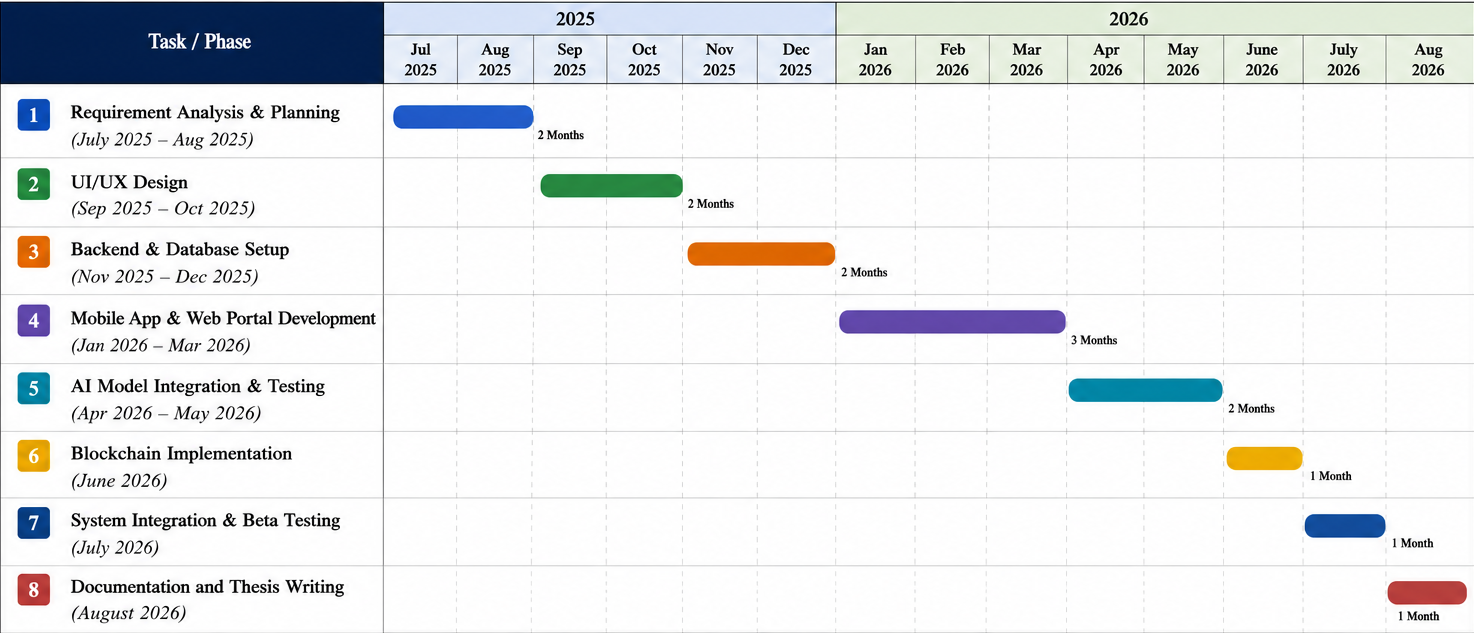
\includegraphics[width=\textwidth]{image/project_gantt_chart.png}
    \caption{Project Timeline and Gantt Chart}
    \label{fig:gantt_chart}
\end{figure}

\vspace{5mm}

\subsection*{Summary}
In summary, the EHealth telemedicine platform was developed with a strong commitment to ethical practices, societal benefit, and technological sustainability. Despite navigating tight budget constraints and complex integration challenges, the project successfully met its milestones by utilizing cost-effective, open-source AI models and an energy-efficient blockchain network. The careful management of design and component limitations resulted in a secure, functional, and socially impactful healthcare solution that strictly protected patient privacy while reducing administrative burdens on medical professionals.